\documentclass[handout]{beamer}  

%Smaller gap at between top and bottom of block when there are displayed equations
\addtobeamertemplate{block begin}{\setlength\abovedisplayskip{0pt}}
{\setlength{\belowdisplayskip}{0pt}}


\usepackage{setspace}
\linespread{1.3}
\usepackage{amssymb, amsmath, amsthm} 
\usepackage{rotating}
\usepackage{multirow}
\usepackage{graphicx}
\usepackage{synttree}
\usepackage{verbatim}
\usepackage{fancybox}
\usepackage{color}
\usepackage{tikz}
\usetikzlibrary{shapes,backgrounds}
\usepackage{hyperref}
\usetikzlibrary{trees}
\newcommand{\p}{\mathbb{P}}
\newcommand{\expect}{\mathbb{E}}


%\setbeamertemplate{blocks}[rounded][shadow=true] 
%gets rid of bottom navigation bars
\setbeamertemplate{footline}{
   \begin{beamercolorbox}[ht=4ex,leftskip=0.3cm,rightskip=0.3cm]{author in head/foot}
%    \usebeamercolor{UniBlue}
    \vspace{0.1cm}
    %\insertshorttitle \ - \insertdate 
    \hfill \insertframenumber / \inserttotalframenumber
   \end{beamercolorbox}
   \vspace*{0.1cm}
} 


%gets rid of navigation symbols
\setbeamertemplate{navigation symbols}{}


%Include or exclude the notes?
%\setbeameroption{show notes}
\setbeameroption{hide notes}

\title[Econ 103]{Economics 103 -- Statistics for Economists} 
\author[F. DiTraglia]{Francis J.\ DiTraglia}
\institute{University of Pennsylvania}
\date{Lecture 12}


\begin{document} 
%%%%%%%%%%%%%%%%%%%%%%%%%%%%%%%%%%%%%%%%



\begin{frame}[plain]
	\titlepage 
	

\end{frame} 


%%%%%%%%%%%%%%%%%%%%%%%%%%%%%%%%%%%%%%%%
%\begin{frame}
%\frametitle{Please Register your Clicker with your \emph{PennKey}}
%Visit the following address:
%\href{http://webreg.turningtechnologies.com/}{\fbox{\texttt{http://webreg.turningtechnologies.com/}}}\\
%and follow the instructions. Enter your \emph{PennKey}, i.e.\ your email prefix, where it asks for your Student ID.
%\end{frame}


%%%%%%%%%%%%%%%%%%%%%%%%%%%%%%%%%%%%%%%%

\begin{frame}
\begin{center}
\Huge Continuous Distributions -- Part II
\end{center}
\end{frame}


%%%%%%%%%%%%%%%%%%%%%%%%%%%%%%%%%%%%%%%%
\begin{frame}
\frametitle{Last Time: Continuous RVs,  Probability As Area}
\begin{block}{Probability Density Function (pdf)}
	\begin{itemize}
		\item $\int_a^b f(x) \; dx = P(a \leq X \leq b)$
		\item $f(x) \geq 0$ for all $x$ in the support
		\item $f(x) \neq P(X=x)$, can be greater than one
	\end{itemize}
\end{block}

\begin{block}{Cumulative Distribution Function}
	\begin{itemize}
		\item $F(x_0) \equiv P(X\leq x_0) =  \int_{-\infty}^{x_0} f(x) \; dx$
		\item First Fundamental Theorem of Calculus: $f(x) = F'(x)$ 
	\end{itemize}
\end{block}


\end{frame}
%%%%%%%%%%%%%%%%%%%%%%%%%%%%%%%%%%%%%%%%
\begin{frame}
\frametitle{Last Time: Uniform$(0,1)$ RV}
\begin{block}{Intuition}
Equally likely to take on any value on its support: $[0,1]$
\end{block}
\begin{block}{Probability Density Function}
	$f(x) = 1$ for $x \in [0,1]$, zero otherwise
\end{block}
\begin{block}{Cumulative Distribution Function}
	$$ F(x_0) = \left\{ \begin{array}{c} 0, x_0 < 0\\ x_0, 0\leq x_0 \leq 1\\ 1, x_0 > 1   \end{array}\right.$$
\end{block}
\end{frame}
%%%%%%%%%%%%%%%%%%%%%%%%%%%%%%%%%%%%%%%%
\begin{frame}
\Huge \begin{center}Key Idea: Probability of Intervals\end{center}
\end{frame}
%%%%%%%%%%%%%%%%%%%%%%%%%%%%%%%%%%%%%%%%
\begin{frame}
\frametitle{What is $P(0.4 \leq X \leq 0.8)$ if $X\sim \mbox{Uniform}(0,1)$? \hfill 
\includegraphics[scale = 0.05]{./images/clicker}}
\centering
	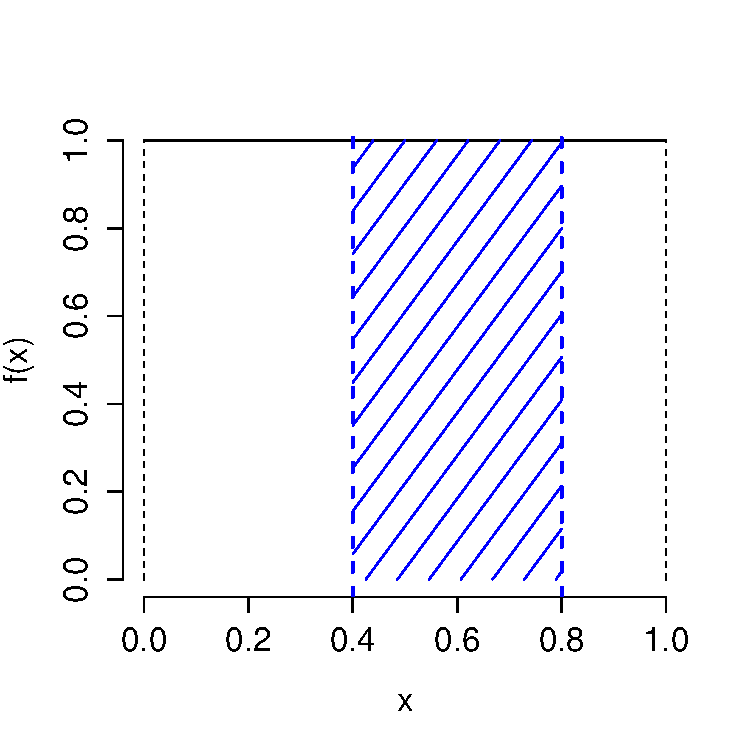
\includegraphics[scale = 0.6]{./images/uniform_density_interval}


\end{frame}
%%%%%%%%%%%%%%%%%%%%%%%%%%%%%%%%%%%%%%%%
\begin{frame}
\frametitle{$F(0.8) = P(X \leq 0.8)$}

\centering
	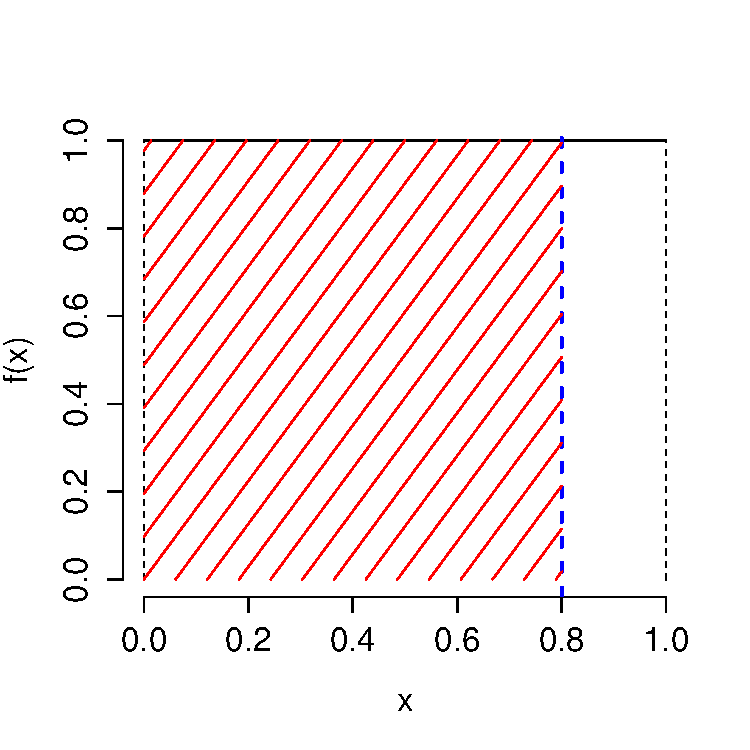
\includegraphics[scale = 0.6]{./images/density_interval_cdf1}

\end{frame}


%%%%%%%%%%%%%%%%%%%%%%%%%%%%%%%%%%%%%%%%
\begin{frame}
\frametitle{$F(0.8) - F(0.4) = $ ?}
\centering
	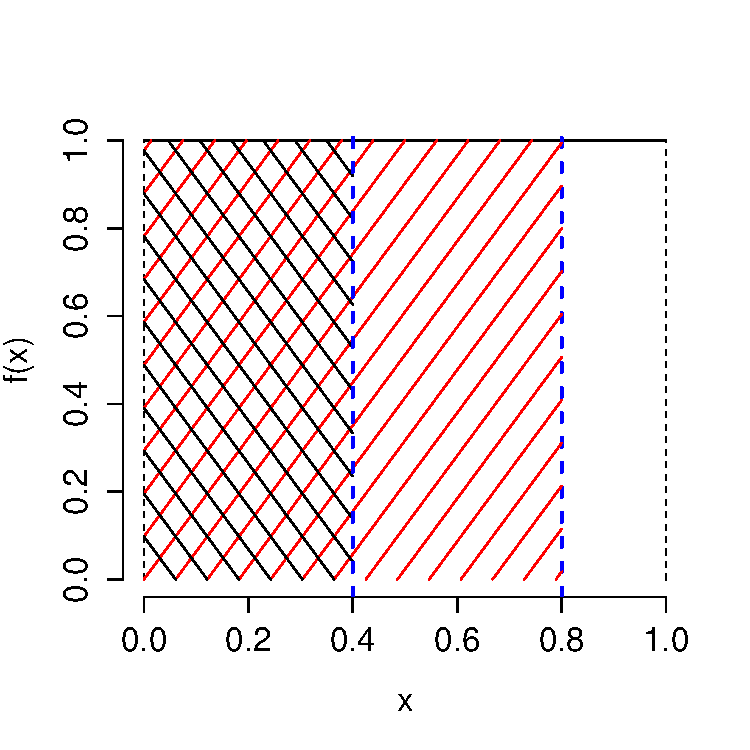
\includegraphics[scale = 0.6]{./images/density_interval_cdf2}

\end{frame}


%%%%%%%%%%%%%%%%%%%%%%%%%%%%%%%%%%%%%%%%
\begin{frame}
\frametitle{$F(0.8) - F(0.4) = P(0.4 \leq X \leq 0.8) = 0.4$}
\centering
	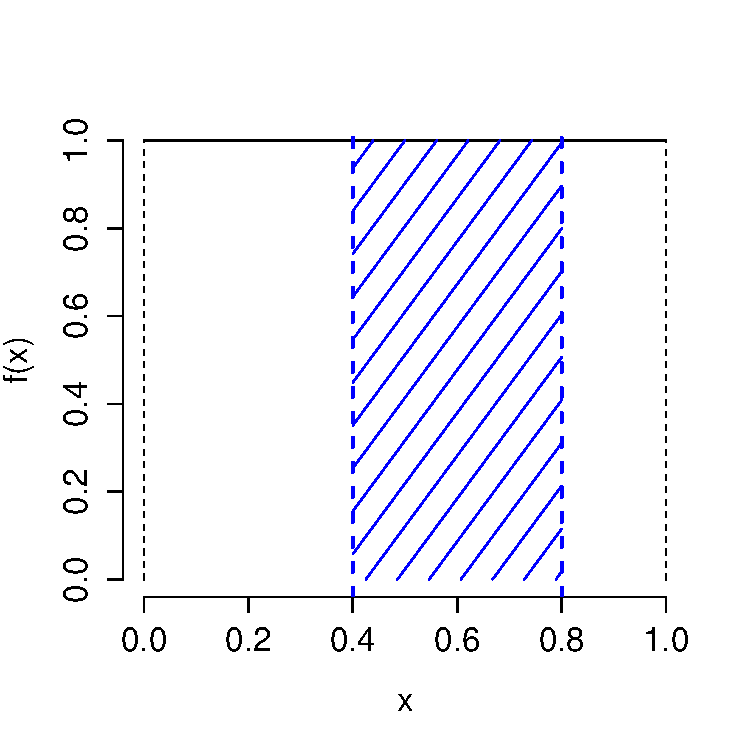
\includegraphics[scale = 0.6]{./images/uniform_density_interval}


\end{frame}
%%%%%%%%%%%%%%%%%%%%%%%%%%%%%%%%%%%%%%%%
\begin{frame}
\frametitle{Probability of Interval for Continuous RV}

$$\boxed{P(a\leq X \leq b) = \int_a^b f(x) \; dx = F(b) - F(a)}$$

\vspace{2em}
\alert{This is just the Second Fundamental Theorem of Calculus.}
\end{frame}
%%%%%%%%%%%%%%%%%%%%%%%%%%%%%%%%%%%%%%%%

\begin{frame}
\frametitle{Expected Value for Continuous RVs}
$$\boxed{\int_{-\infty}^\infty x f(x) \; dx  }$$

\vspace{2em}
\alert{Remember: Integrals Replace Sums!}
\end{frame}

%%%%%%%%%%%%%%%%%%%%%%%%%%%%%%%%%%%%%%%%
\begin{frame}
\frametitle{Example: Uniform(0,1) Random Variable \hfill 
\includegraphics[scale = 0.05]{./images/clicker}}
\begin{eqnarray*}
	E[X] &=&  \int_{-\infty}^\infty x f(x) \; dx =\pause  \int_{0}^1 x \cdot 1 \; dx \\ \\
		&=& \pause \left.\frac{x^2}{2}\right|_0^1 =\pause  1/2  - 0 = 1/2
\end{eqnarray*}
\end{frame}
%%%%%%%%%%%%%%%%%%%%%%%%%%%%%%%%%%%%%%%%
\begin{frame}
\frametitle{Expected Value of a Function of a Continuous RV}
	$$\boxed{E[g(X)] = \int_{-\infty}^\infty g(x) f(x) \; dx}$$
\end{frame}


%%%%%%%%%%%%%%%%%%%%%%%%%%%%%%%%%%%%%%%%

\begin{frame}
\frametitle{Example: Uniform$(0,1)$ RV}
	\begin{eqnarray*}
	E[X^2] &=& \pause \int_{-\infty}^\infty x^2 f(x) \; dx = \pause \int_0^1 x^2 \cdot 1 \; dx\\ \\
		&=& \left. \frac{x^3}{3}\right|_0^1 = \pause 1/3
	\end{eqnarray*}
\end{frame}


%%%%%%%%%%%%%%%%%%%%%%%%%%%%%%%%%%%%%%%%

\begin{frame}
Once we have defined expected value for continuous RVs, we can use everything we know about variance, covariance, etc.\ from discrete RVs!
\end{frame}

%%%%%%%%%%%%%%%%%%%%%%%%%%%%%%%%%%%%%%%%
\begin{frame}
\frametitle{Variance of Continuous RV}

$$\boxed{Var(X) = \int_{-\infty}^{\infty} (x - \mu)^2 f(x) \; dx}$$

\vspace{2em}
where
$$\mu = E[X]=\int_{-\infty}^\infty x f(x) \; dx $$

\vspace{2em}
\alert{Shortcut formula still holds for continuous RVs!}
	$$Var(X) = E[X^2] - \left(E[X]\right)^2$$
\end{frame}
%%%%%%%%%%%%%%%%%%%%%%%%%%%%%%%%%%%%%%%%

\begin{frame}
\frametitle{Example: Uniform(0,1) Random Variable \hfill 
\includegraphics[scale = 0.05]{./images/clicker}}
\begin{eqnarray*}
 Var(X) &=& E\left[ \left( X - E[X] \right)^2\right] = E[X^2] - \left(E[X]\right)^2\\ \pause
 	&=& 1/3  - (1/2)^2\\ \pause
 	&=& 1/12 \\
 	&\approx& 0.083
\end{eqnarray*}
\end{frame}

%%%%%%%%%%%%%%%%%%%%%%%%%%%%%%%%%%%%%%%%
\begin{frame}
\frametitle{Much More Complicated Without the Shortcut Formula!}
\begin{eqnarray*}
 Var(X) &=& E\left[ \left( X - E[X] \right)^2\right] = \int_{-\infty}^{\infty} (x - \mu)^2 f(x) \; dx\\ \\
 	&=&\int_{0}^{1} (x -1/2)^2 \cdot 1 \; dx = \int_{0}^{1} (x^2  - x + 1/4) \; dx \\ \\
 		&=& \left. \left(\frac{x^3}{3} - \frac{x^2}{2} + \frac{x}{4}  \right)\right|_0^1 = 1/3 - 1/2 + 1/4\\ \\ 
 			&=& 4/12 - 6/12 + 3/12 = 1/12
\end{eqnarray*}
\end{frame}

%%%%%%%%%%%%%%%%%%%%%%%%%%%%%%%%%%%%%%%%
\begin{frame}
\frametitle{We're Won't Say More About These, But Just So You're Aware of Them...}

\begin{block}{Joint Density}
$ \displaystyle P(a\leq X \leq b \cap c\leq Y \leq d) = \int_c^d \int_a^b f(x,y) \; dxdy$
\end{block}
\begin{block}{Marginal Densities}
$f_X(x) = \int_{-\infty}^\infty f(x,y)\; dy$, $\;\;\;\;\;\;\; f_Y(y) = \int_{-\infty}^\infty f(x,y)\; dx$
\end{block}
\begin{block}{Independence in Terms of Joint and Marginal Densities}
$f_{XY}(x,y) = f_X(x)f_Y(y)$
\end{block}
\begin{block}{Conditional Density}
$f_{Y|X} = f_{XY}(x,y)/f_X(x)$
\end{block}

\end{frame}

%%%%%%%%%%%%%%%%%%%%%%%%%%%%%%%%%%%%%%%%
\begin{frame}

\huge We've now covered everything on the RV Handout posted on Piazza.

\end{frame}
%%%%%%%%%%%%%%%%%%%%%%%%%%%%%%%%%%%%%%%%
\begin{frame}
\Huge \begin{center}
The Most Important RV of All
\end{center}

\end{frame}
%%%%%%%%%%%%%%%%%%%%%%%%%%%%%%%%%%%%%%%%
\begin{frame}
\frametitle{Normal Random Variable}
\begin{block}{Notation: $X \sim N(\mu, \sigma^2)$}
Parameters: $\mu = E[X]$, $\sigma^2 = Var(X)$\\ Support:  $(-\infty, +\infty)$
\end{block}


\begin{block}{Probability Density Function}
	$$ f(x) = \frac{1}{\sqrt{2\pi \sigma^2}} \exp \left\{ - \frac{1}{2} \left(\frac{x - \mu}{\sigma} \right)^2 \right\}$$
\end{block}


\begin{block}{No Explicit Formula for CDF (use computer instead)}
	$$F(x_0) = \int_{-\infty}^{x_0}  \frac{1}{\sqrt{2\pi \sigma^2}} \exp \left\{ - \frac{1}{2} \left(\frac{x - \mu}{\sigma} \right)^2 \right\} \; dx$$
\end{block}
\end{frame}

%%%%%%%%%%%%%%%%%%%%%%%%%%%%%%%%%%%%%%%%


\begin{frame}
\frametitle{Normal PDF Centered at the Mean (Here $\mu = 0$, $\sigma^2 = 1$)}

\begin{figure}
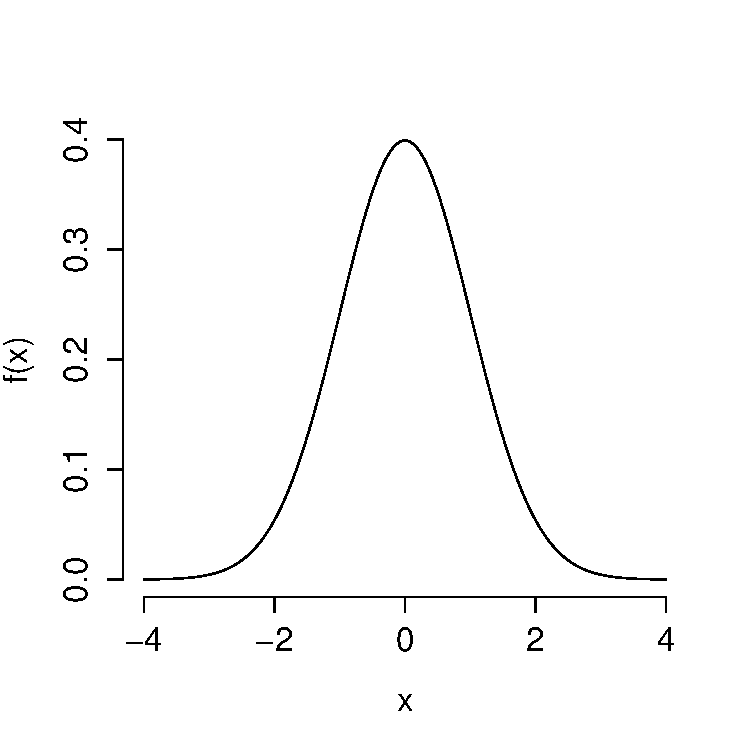
\includegraphics[scale = 0.65]{./images/std_normal_PDF}
\end{figure}
\end{frame}

%%%%%%%%%%%%%%%%%%%%%%%%%%%%%%%%%%%%%%%%



\begin{frame}
\frametitle{Normal CDF ($\mu = 0$, $\sigma^2 = 1$)}

\begin{figure}
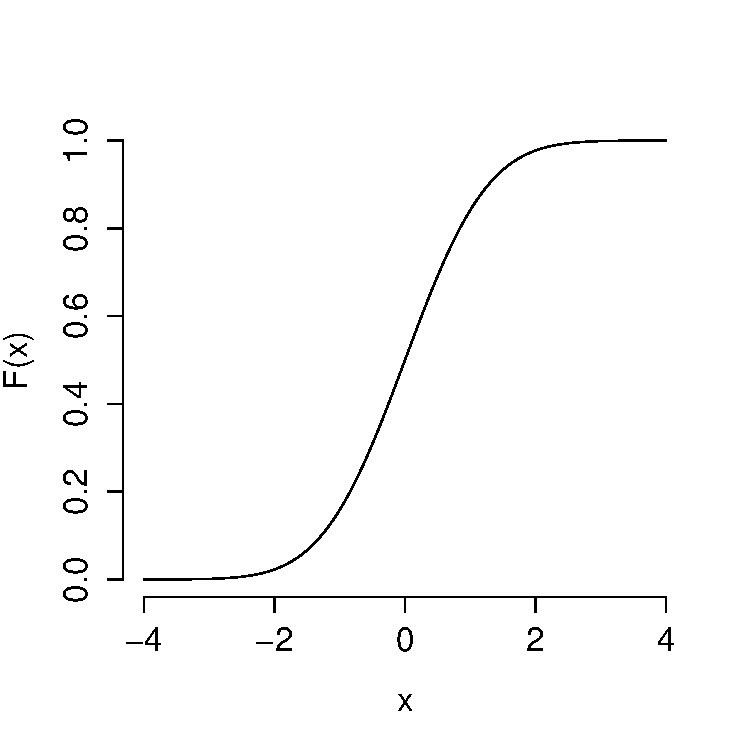
\includegraphics[scale = 0.62]{./images/std_normal_CDF}
\end{figure}
\end{frame}

%%%%%%%%%%%%%%%%%%%%%%%%%%%%%%%%%%%%%%%%

\begin{frame}
	\frametitle{\href{http://glimmer.rstudio.com/fditraglia/normal_cdf/}{http://glimmer.rstudio.com/fditraglia/normal\_cdf/}}

\begin{figure}
	\fbox{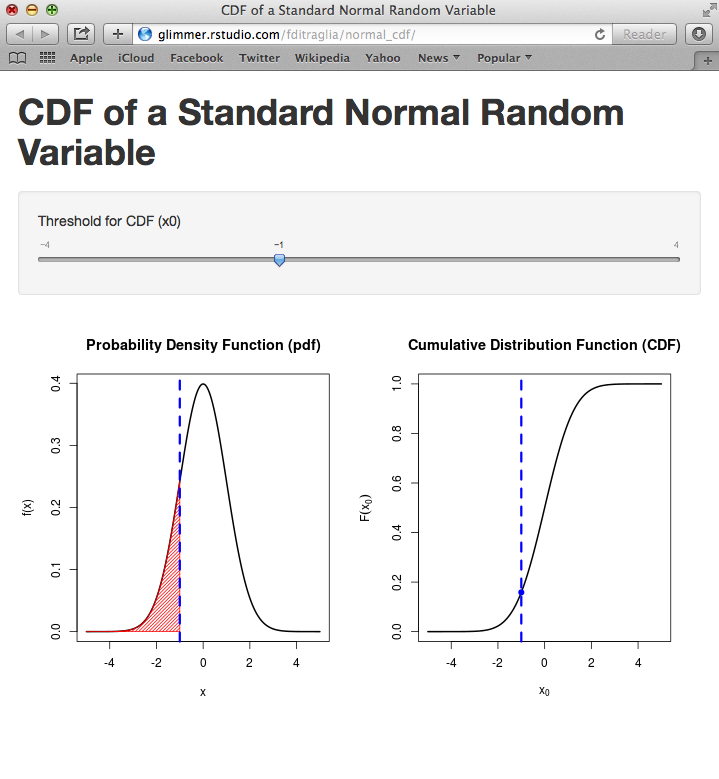
\includegraphics[scale = 0.2]{./images/normal_cdf_screenshot}}
\end{figure}

\end{frame}

%%%%%%%%%%%%%%%%%%%%%%%%%%%%%%%%%%%%%%%%




\begin{frame}
\frametitle{Different Means, Same Variance}

\begin{figure}
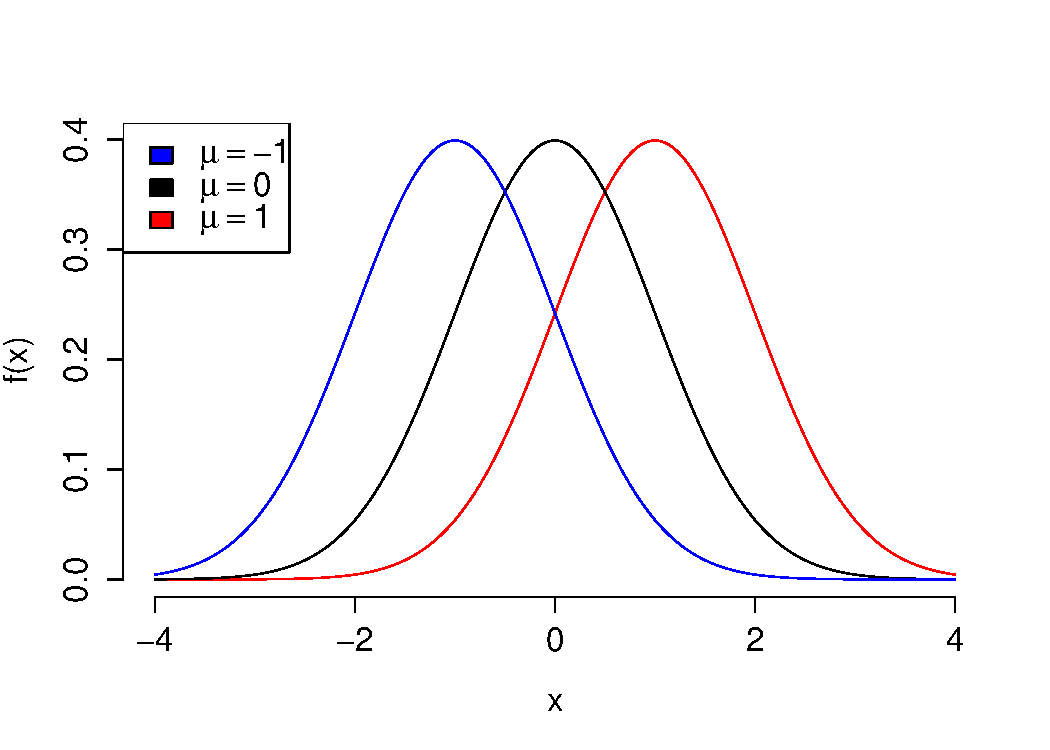
\includegraphics[scale = 0.65]{./images/normal_means}
\end{figure}
\end{frame}

%%%%%%%%%%%%%%%%%%%%%%%%%%%%%%%%%%%%%%%%


\begin{frame}
\frametitle{Same Mean, Different Variances}

\begin{figure}
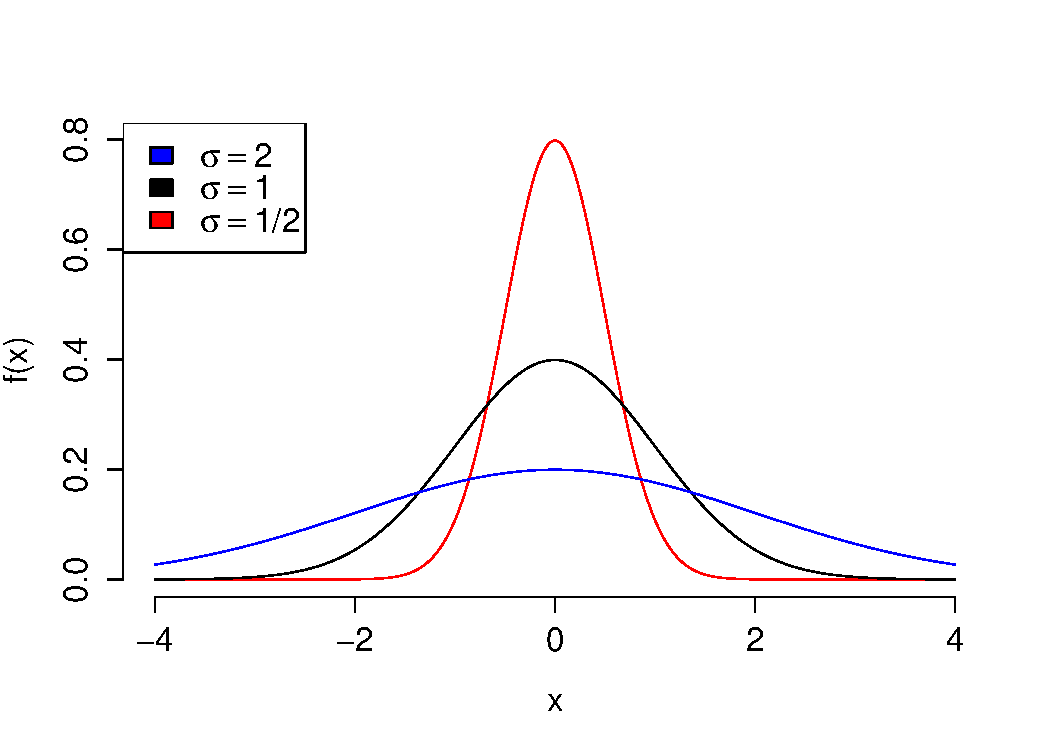
\includegraphics[scale = 0.62]{./images/normal_std_devs}
\end{figure}
\end{frame}

%%%%%%%%%%%%%%%%%%%%%%%%%%%%%%%%%%%%%%%%


\begin{frame}
\frametitle{Linear Function of Normal RV is a Normal RV}


Suppose that $X \sim N(\mu, \sigma^2)$. Then if $a$ and $b$ constants,
$$\boxed{a + bX \sim N(a + b\mu, b^2 \sigma^2)}$$


\begin{block}{Important}
	\begin{itemize}
		\item  Using what know know about expectations of linear functions, no surprise what mean and variance are.
		\item Surprise is that the linear combination is \emph{\alert{normal}}
		\item Linear trans.\ does not preserve, e.g.,  Bernoulli or Binomial.
	\end{itemize}
\end{block}

\end{frame}

%%%%%%%%%%%%%%%%%%%%%%%%%%%%%%%%%%%%%%%%
\begin{frame}
\frametitle{Example \hfill 
\includegraphics[scale = 0.05]{./images/clicker}}
Suppose $X \sim N(\mu, \sigma^2)$ and let $Z = (X -\mu)/\sigma$. What is the distribution of $Z$?

\begin{enumerate}[(a)]
	\item $N(\mu, \sigma^2)$
	\item $N(\mu, \sigma)$
	\item $N(0, \sigma^2)$
	\item  $N(0, \sigma)$
	\item $N(0,1)$
\end{enumerate}
\end{frame}



%%%%%%%%%%%%%%%%%%%%%%%%%%%%%%%%%%%%%%%%
\begin{frame}
\begin{figure}
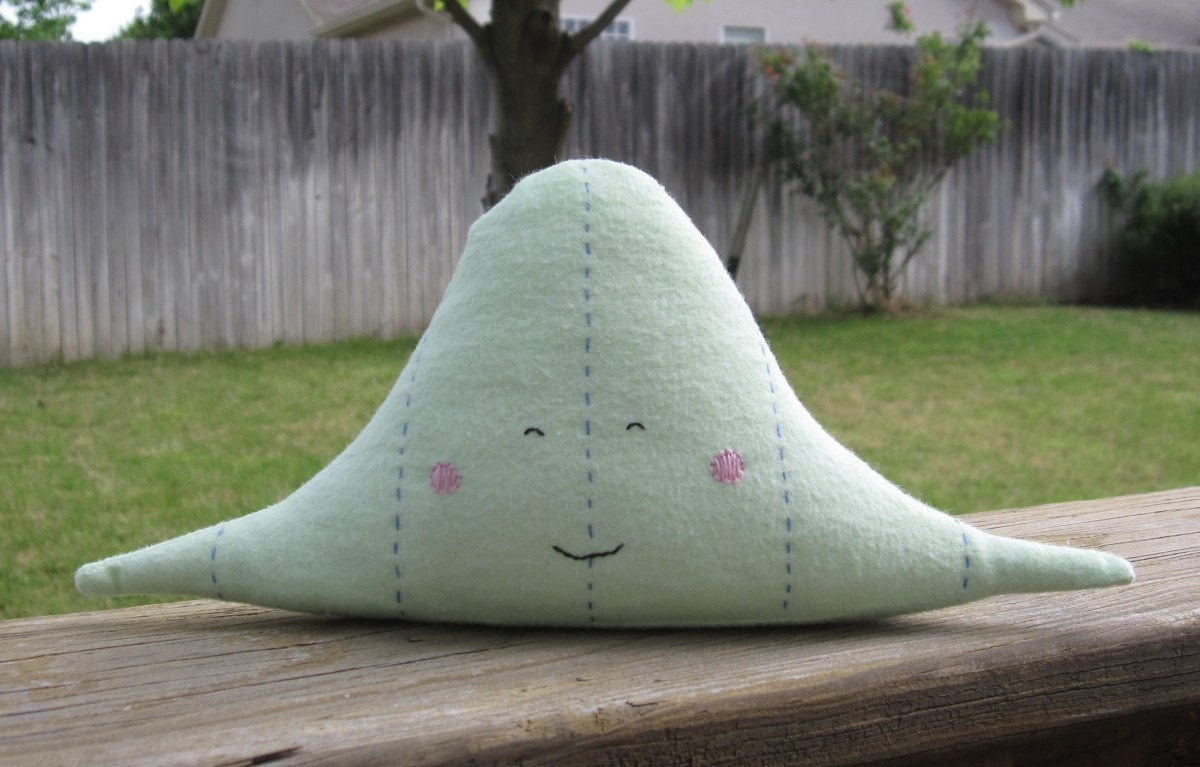
\includegraphics[scale = 0.2]{./images/normal_etsy1}
\caption{Standard Normal Distribution (PDF)}
\end{figure}
\end{frame}

%%%%%%%%%%%%%%%%%%%%%%%%%%%%%%%%%%%%%%%%
\begin{frame}
\frametitle{Standard Normal Distribution: $N(0,1)$}
\begin{figure}
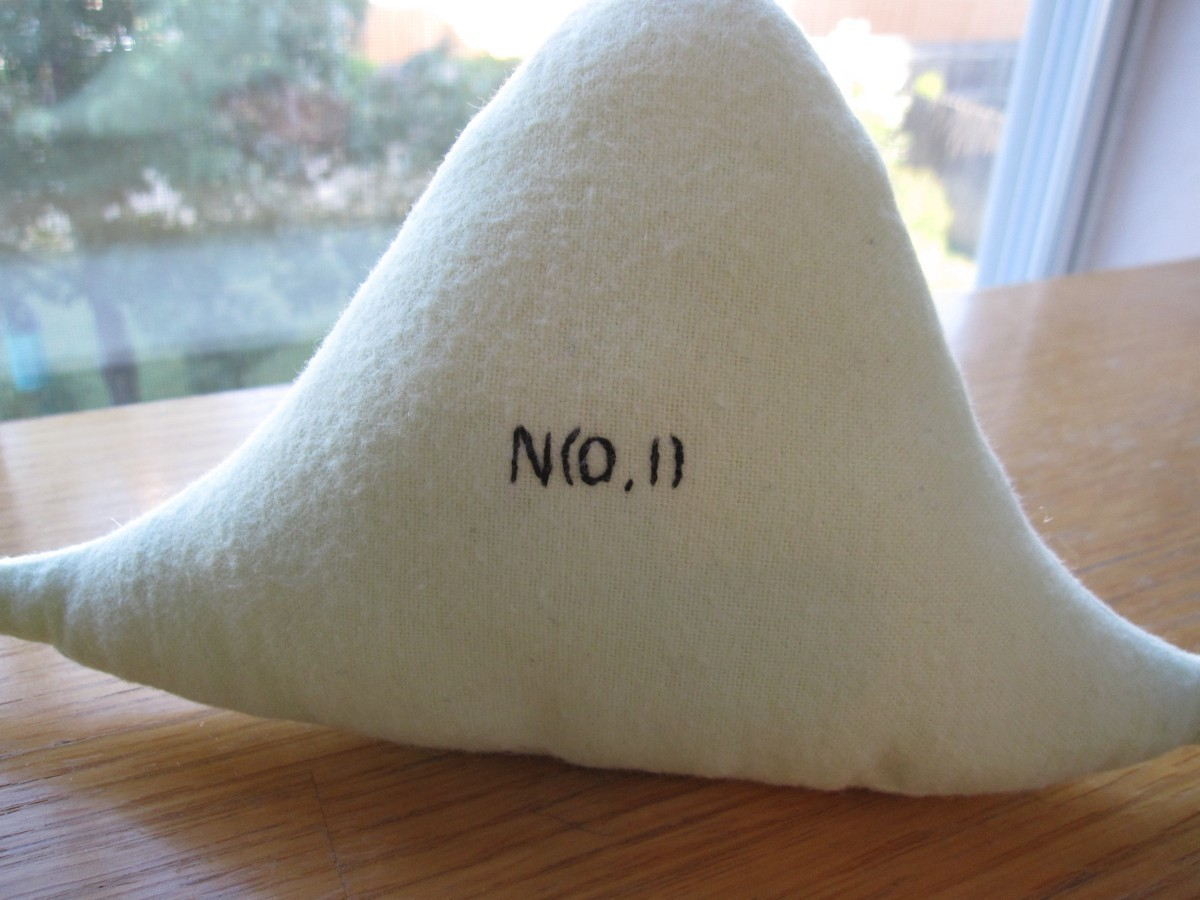
\includegraphics[scale = 0.2]{./images/normal_etsy2}
\end{figure}
\end{frame}
%%%%%%%%%%%%%%%%%%%%%%%%%%%%%%%%%%%%%%%%
\begin{frame}
\frametitle{Standard Normal Distribution: $N(0,1)$}
Mean = 0, Variance = Standard Deviation = 1
	$$f(x) = \frac{1}{\sqrt{2\pi}} e^{-x^2/2}$$

Special symbol for Standard Normal CDF (no closed form):
	$$\Phi(x_0) = \int_{-\infty}^{x_0}\frac{1}{\sqrt{2\pi}} e^{-x^2/2}\; dx $$
	
R Command: $\Phi(x_0) =$\texttt{pnorm()}
\end{frame}



%%%%%%%%%%%%%%%%%%%%%%%%%%%%%%%%%%%%%%%%
%\begin{frame}
%\begin{figure}
%
\includegraphics[scale = 0.2]{./images/normal_etsy_pumpkin}
%\caption{Standard Normal PDF -- Halloween Edition}
%\end{figure}
%\end{frame}
%%%%%%%%%%%%%%%%%%%%%%%%%%%%%%%%%%%%%%%%
%\begin{frame}
%\begin{figure}
%
\includegraphics[scale = 0.2]{./images/normal_etsy_bat}
%\caption{Standard Normal PDF -- Alternate Halloween Edition}
%\end{figure}
%\end{frame}
%%%%%%%%%%%%%%%%%%%%%%%%%%%%%%%%%%%%%%%%
\begin{frame}
\frametitle{Where does the Empirical Rule come from?}

\begin{block}{Empirical Rule}
Approximately 68\% of observations within $\mu\pm \sigma$\\
Approximately 95\% of observations within $\mu\pm 2 \sigma$\\
Nearly all observations within $\mu\pm 3 \sigma$\\
\end{block}
\end{frame}

%%%%%%%%%%%%%%%%%%%%%%%%%%%%%%%%%%%%%%%%

\begin{frame}
\frametitle{Middle 68\% of $N(0,1) \Rightarrow$ approx.\ $(-1,1)$}
\begin{figure}
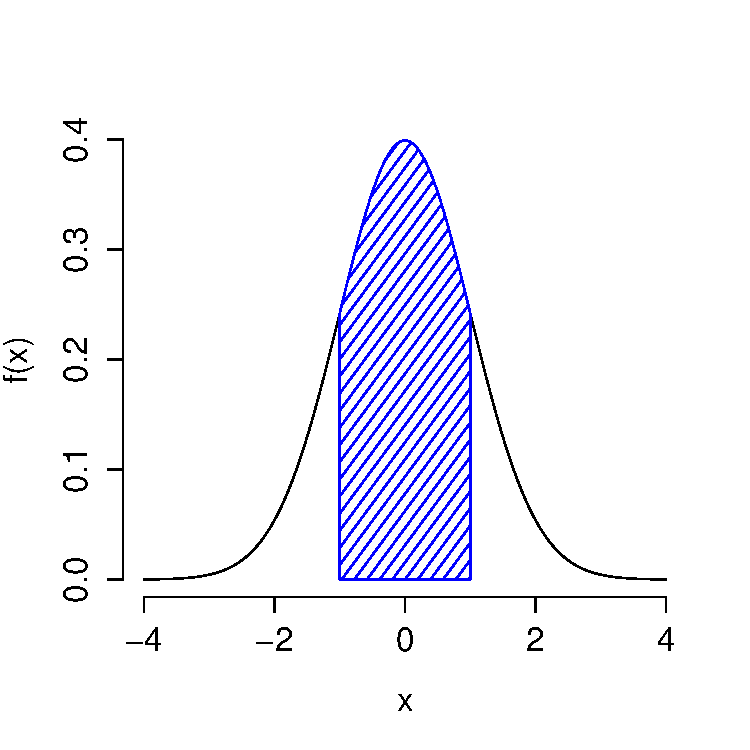
\includegraphics[scale = 0.65]{./images/normal_middle68}
\end{figure}
\end{frame}

%%%%%%%%%%%%%%%%%%%%%%%%%%%%%%%%%%%%%%%%

\begin{frame}
\frametitle{Middle 95\% of $N(0,1)\Rightarrow$ approx.\ $(-2,2)$}

\begin{figure}
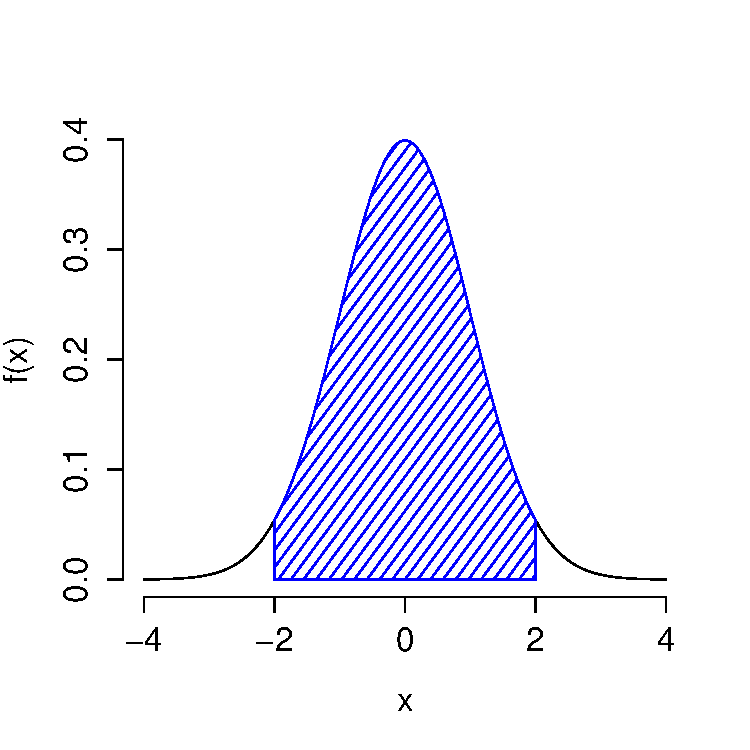
\includegraphics[scale = 0.65]{./images/normal_middle95}
\caption{PDF for t-Distribution}
\end{figure}
\end{frame}
%%%%%%%%%%%%%%%%%%%%%%%%%%%%%%%%%%%%%%%%
\begin{frame}
\frametitle{More Formally...}
$$\int_{-1}^1 \frac{1}{\sqrt{2\pi}} e^{-x^2/2}\; dx  \approx 0.68$$
\vspace{2em}
$$\int_{-2}^2 \frac{1}{\sqrt{2\pi}} e^{-x^2/2}\; dx  \approx 0.95$$
\begin{alertblock}{But how do we know this?}\end{alertblock}
\end{frame}
%%%%%%%%%%%%%%%%%%%%%%%%%%%%%%%%%%%%%%%%

\begin{frame}
\frametitle{$\Phi(1) =$\texttt{pnorm(1)}$\approx 0.84$}

\begin{figure}
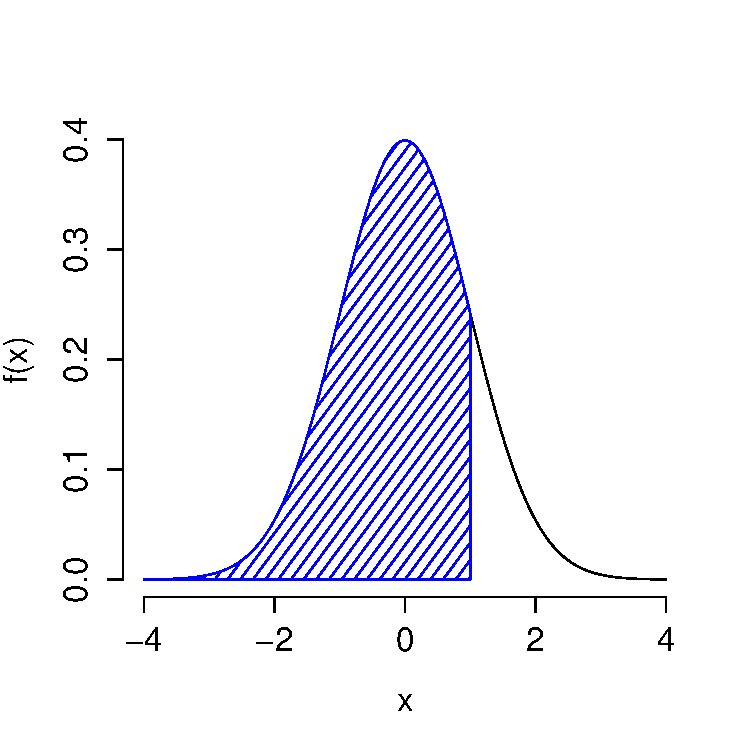
\includegraphics[scale = 0.65]{./images/middle68_1}
\end{figure}
\end{frame}
%%%%%%%%%%%%%%%%%%%%%%%%%%%%%%%%%%%%%%%%
\begin{frame}
\frametitle{$\Phi(1) - \Phi(-1) =$\texttt{pnorm(1) - pnorm(-1)}$\approx 0.84 - 0.16$}
\begin{figure}
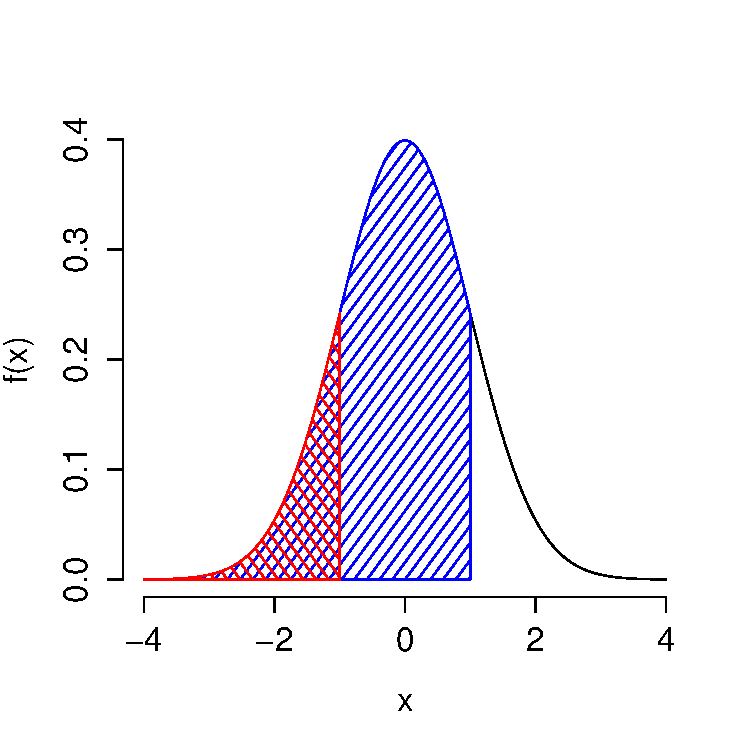
\includegraphics[scale = 0.65]{./images/middle68_2}
\end{figure}
\end{frame}
%%%%%%%%%%%%%%%%%%%%%%%%%%%%%%%%%%%%%%%%
\begin{frame}
\frametitle{$\Phi(1) - \Phi(-1) =$\texttt{pnorm(1) - pnorm(-1)}$\approx 0.68$}
\begin{figure}
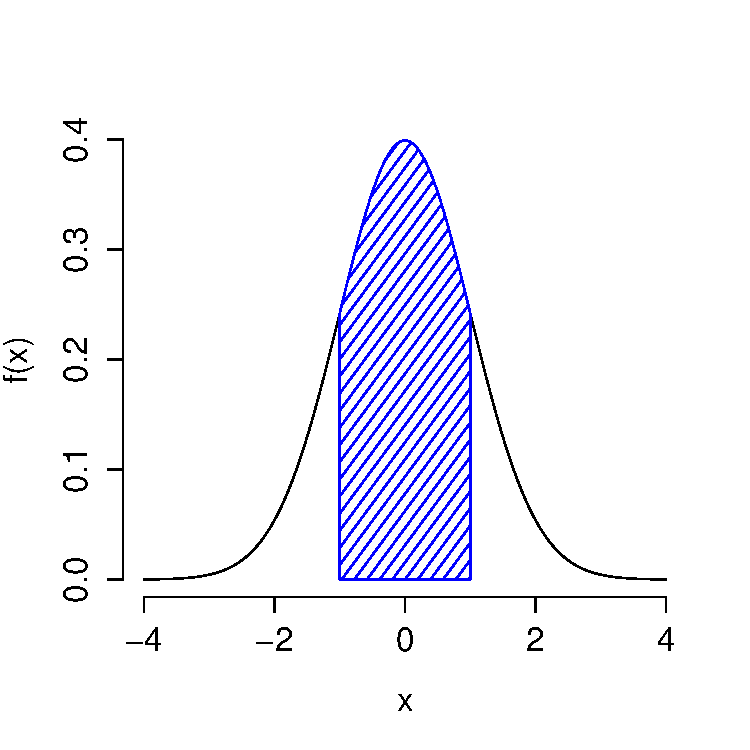
\includegraphics[scale = 0.65]{./images/middle68_3}
\end{figure}
\end{frame}
%%%%%%%%%%%%%%%%%%%%%%%%%%%%%%%%%%%%%%%%
\begin{frame}
\frametitle{Suppose $X \sim N(0,1)$}
\begin{eqnarray*}
	P(-2 \leq X \leq 2) &=& \Phi(2) - \Phi(-2) \\
		&=& \mbox{\texttt{pnorm(2) - pnorm(-2)}}\\
		&\approx& 0.95
\end{eqnarray*}
\pause
\begin{eqnarray*}
	P(-3 \leq X \leq 3) &=& \Phi(3) - \Phi(-3) \\
		&=& \mbox{\texttt{pnorm(3) - pnorm(-3)}}\\
		&\approx& 1
\end{eqnarray*}

\end{frame}
%%%%%%%%%%%%%%%%%%%%%%%%%%%%%%%%%%%%%%%%
%%%%%%%%%%%%%%%%%%%%%%%%%%%%%%%%%%%%%%%%
\begin{frame}
\frametitle{What if $X \sim N(\mu, \sigma^2)$?}
\begin{eqnarray*}
	P(X \leq a) &=& \pause P(X - \mu \leq a - \mu)\\\\
		&=& \pause P\left( \frac{X-\mu}{\sigma} \leq \frac{a - \mu}{\sigma} \right)\\\\
		&=&\pause  P\left(Z \leq  \frac{a - \mu}{\sigma}\right)
\end{eqnarray*}
Where $Z$ is a standard normal random variable, i.e.\ $N(0,1)$.
\end{frame}


%%%%%%%%%%%%%%%%%%%%%%%%%%%%%%%%%%%%%%%%
\begin{frame}
\frametitle{
\includegraphics[scale = 0.05]{./images/clicker}}
Which of these equals $P\left(Z \leq (a-\mu)/\sigma\right)$ if $Z\sim N(0,1)$?
	\begin{enumerate}[(a)]
		\item $\Phi(a)$
		\item $1 - \Phi(a)$
		\item $\Phi(a)/\sigma - \mu$
		\item $\Phi\left(\frac{a - \mu}{\sigma}  \right)$
		\item None of the above.
	\end{enumerate}
\end{frame}
%%%%%%%%%%%%%%%%%%%%%%%%%%%%%%%%%%%%%%%%

\begin{frame}
\frametitle{What if $X \sim N(\mu, \sigma^2)$?}
\begin{eqnarray*}
	P(X \leq a) &=&\ P(X - \mu \leq a - \mu)\\\\
		&=& P\left( \frac{X-\mu}{\sigma} \leq \frac{a - \mu}{\sigma} \right)\\\\
		&=& P\left(Z \leq  \frac{a - \mu}{\sigma}\right)\\
		&=&\alert{\Phi\left(\frac{a - \mu}{\sigma}  \right)}\\
		&=&\alert{ \mbox{\texttt{pnorm}}((a-\mu)/\sigma)}
\end{eqnarray*}
Where $Z$ is a standard normal random variable, i.e.\ $N(0,1)$.
\end{frame}


%%%%%%%%%%%%%%%%%%%%%%%%%%%%%%%%%%%%%%%%
\begin{frame}
\frametitle{Suppose $X \sim N(\mu, \sigma^2)$ \hfill 
\includegraphics[scale = 0.05]{./images/clicker}}
Which of these is $P(X \geq b)$?
\begin{enumerate}[(a)]
	\item $\Phi(b)$
	\item $1 - \Phi\left( \frac{b - \mu}{\sigma} \right)$
	\item $1 - \Phi(b)$
	\item $1 - \left(\Phi(b)/\sigma - \mu\right)$
\end{enumerate}

\end{frame}
\begin{frame}
\frametitle{Suppose $X \sim N(\mu, \sigma^2)$}
\begin{eqnarray*}
	P(X \geq b) &=&\pause 1 - P(X\leq b) =\pause 1 - P\left( \frac{X-\mu}{\sigma} \leq \frac{b-\mu}{\sigma} \right) \\ \\
	&=&\pause 1 - P\left( Z \leq \frac{b-\mu}{\sigma} \right) = 1 - \Phi\left( \frac{b-\mu}{\sigma} \right)\\ \\
	&=&\pause 1 -\mbox{\texttt{pnorm}}((b-\mu)/\sigma)
\end{eqnarray*}
Where $Z$ is a standard normal random variable.
\end{frame}
%%%%%%%%%%%%%%%%%%%%%%%%%%%%%%%%%%%%%%%%
\begin{frame}
\frametitle{Suppose $X \sim N(\mu, \sigma^2)$}


\begin{eqnarray*}
	P(a \leq X \leq b) &=& \pause P\left( \frac{a - \mu}{\sigma} \leq \frac{X - \mu}{\sigma} \leq \frac{b-\mu}{\sigma} \right)\\ \\ 
	&=& \pause P\left( \frac{a - \mu}{\sigma} \leq Z \leq \frac{b-\mu}{\sigma} \right)\\ \\ 
	&=& \pause \Phi\left( \frac{b-\mu}{\sigma}\right) - \Phi\left( \frac{a - \mu}{\sigma}\right)\\ \\
	&=&\pause \mbox{\texttt{pnorm}}((b-\mu)/\sigma) -  \mbox{\texttt{pnorm}}((a-\mu)/\sigma)
\end{eqnarray*}
Where $Z$ is a standard normal random variable.
\end{frame}
%%%%%%%%%%%%%%%%%%%%%%%%%%%%%%%%%%%%%%%%
\begin{frame}
\frametitle{Suppose $X \sim N(\mu, \sigma^2)$\hfill 
\includegraphics[scale = 0.05]{./images/clicker}}
What is $P(\mu - \sigma \leq X \leq \mu + \sigma)$?
\end{frame}

%%%%%%%%%%%%%%%%%%%%%%%%%%%%%%%%%%%%%%%%
\begin{frame}
\frametitle{Suppose $X \sim N(\mu, \sigma^2)$}

\begin{eqnarray*}
P(\mu - \sigma \leq X \leq \mu + \sigma) &=&\pause P\left( -1 \leq \frac{X-\mu}{\sigma} \leq 1\right)\\ \\
	&=&\pause P\left( -1 \leq Z \leq 1\right)\\
	&=&\pause \Phi(1) - \Phi(-1)\\
	&=&\pause \mbox{\texttt{pnorm(1)}} -  \mbox{\texttt{pnorm(-1)}}\\
	&\approx& 0.68
\end{eqnarray*}
\end{frame}

%%%%%%%%%%%%%%%%%%%%%%%%%%%%%%%%%%%%%%%%

\begin{frame}
\frametitle{Suppose $X \sim N(\mu, \sigma^2)$\hfill 
\includegraphics[scale = 0.05]{./images/clicker}}
What is $P(\mu - 2\sigma \leq X \leq \mu + 2\sigma)$?
\end{frame}

%%%%%%%%%%%%%%%%%%%%%%%%%%%%%%%%%%%%%%%%
\begin{frame}
\frametitle{Suppose $X \sim N(\mu, \sigma^2)$}

\begin{eqnarray*}
P(\mu - 2\sigma \leq X \leq \mu + 2\sigma) &=&\pause P\left( -2 \leq \frac{X-\mu}{\sigma} \leq 2\right)\\ \\
	&=&\pause P\left( -2 \leq Z \leq 2\right)\\
	&=&\pause \Phi(2) - \Phi(-2)\\
	&=&\pause \mbox{\texttt{pnorm(2)}} -  \mbox{\texttt{pnorm(-2)}}\\
	&\approx& 0.95
\end{eqnarray*}
\end{frame}


%%%%%%%%%%%%%%%%%%%%%%%%%%%%%%%%%%%%%%%%


\end{document}